\chapter{Plasma分布式内存存储架构和性能分析}

\section{Ray架构简介}

\autoref{fig:ray_arch}\cite{ray_whitepaper}
展示了分布式计算框架Ray的整体架构,并展示了分布式内存对象存储Plasma在其中的位置和角色:

\begin{figure}[h] 
    \centering
    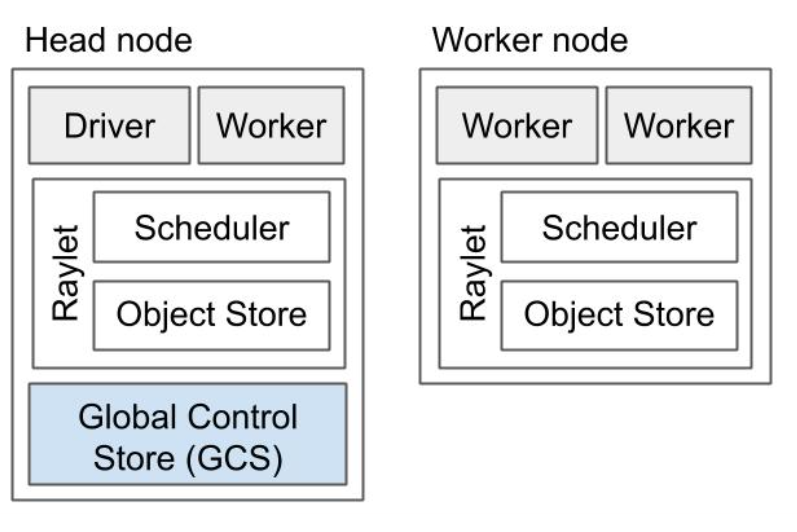
\includegraphics[width=0.6\textwidth]{image/chap02/ray_arch.png}
    \caption{Ray计算架构}
    \label{fig:ray_arch}
\end{figure}

\textbf{Ray架构简介:}
一个Ray集群由主节点(Head Node)和工作节点(Worker Node)构成。主节点上运行驱动(Driver)进程,即编写了Ray函数和其他逻辑(如\autoref{sec:background}中代码片段)的Python程序;另外,还运行着全局控制存储(Global Control Store,GCS):
该数据库存放着Ray集群范围的关键配置信息。此外,所有节点都运行着Ray集群的核心中间件:Raylet。Raylet主要由调度器和对象存储构成——调度器负责将Driver进程解析出的任务调度到集群的合适节点中运行;
对象存储就是Plasma数据库,存放着计算所产生的数据——包括任务运行所依赖的输入数据和所产生的输出数据。

\textbf{Plasma工作机制:}
Plasma对象存储运行在Ray集群的所有节点上。\autoref{fig:object_fetch}\cite{ray_whitepaper}
展示了Ray驱动Plasma对象存储的基本机制:当Ray任务需要获取一个对象x以执行任务时,它将调用“ray.get”方法获取对象。如果该对象存放在本节点的Plasma存储中,后者将通过进程间通信(IPC)将对象传递给任务进程。否则,
它首先需要以下图所示的方式从其他节点拉取数据:

\begin{enumerate}
    \item 当前的Ray实现通过“拥有(Ownership\cite{wang2021ownership})”机制管理对象的存储位置。Plasma向拥有该数据的进程(Owner)查询数据在集群中的位置。
    \item Plasma向该节点的另一个(位于节点2的)Plasma进程发起对象请求。
    \item Plasma将数据传输并保存到本地。
\end{enumerate}

\begin{figure}[h] 
    \centering
    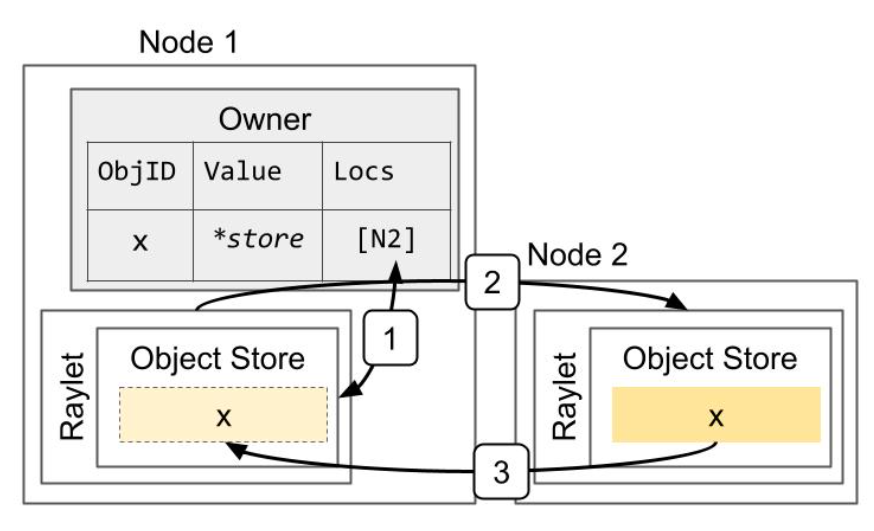
\includegraphics[width=0.6\textwidth]{image/chap02/object_fetch.png}
    \caption{Plasma工作机制}
    \label{fig:object_fetch}
\end{figure}

\textbf{Plasma对象的不可变特性:}Ray以及Plasma中的数据对象均是不可变的(Immutable)。这意味着,对已有内存对象做出任何修改都将生成一个全新的对象,并赋予不同的标识符。
Plasma的这一特性和Redis等键值对数据库有很大的不同:配合引用计数(Reference Counting)机制,不可变数据对象是分布式计算框架中常采用的一种设计。这对计算框架的设计有诸多好处:

\begin{enumerate}
    \item 避免复杂的并发读写机制
    \item 简化任务和资源调度机制的实现
    \item 简化错误发现和恢复机制的实现
\end{enumerate}

不过,不可变特性并不符合“零拷贝”的性能优化原则,因此会对计算框架的性能造成负担:由于对象存储之间、对象存储和任务进程之间的通信,对象传输机制存在较大的固定延迟,因此Ray频繁创建、移动小对象会显著影响其整体性能。

目前,Ray的实际实现中规定仅有大于100KiB大小
\cite{ray_whitepaper}的对象通过Plasma对象存储实现集群共享——
任务进程将更小的数据直接存放在进程的预留空间内,并通过将这些数据内嵌(inline)在RPC调用的参数中实现传递。这一实现策略指引我们在接下来的性能测试和分析中关注Plasma在大对象传输中的性能瓶颈。

\section{Plasma架构分析}

Plasma分布式存储架构由多个进程组成。通过将控制面、数据面上的任务解耦到不同的进程,我们可以较为方便地对其软件架构进行改进。
\autoref{fig:plasma_arch}展示了Plasma集群的组织结构。

\begin{figure}[h] 
    \centering
    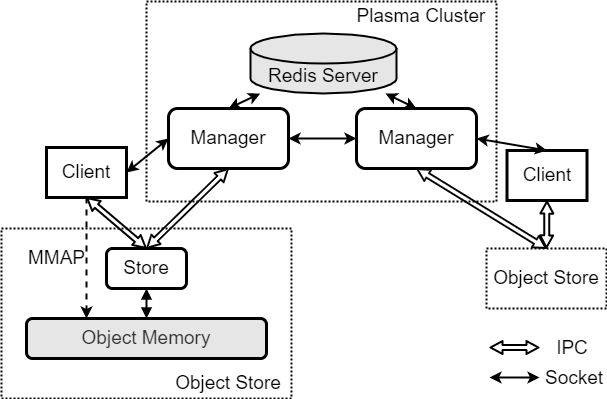
\includegraphics[width=0.75\textwidth]{image/chap02/plasma_arch.png}
    \caption{Plasma存储架构}
    \label{fig:plasma_arch}
\end{figure}

\subsection{Plasma对象存储架构}

\autoref{fig:plasma_arch}中左下方部分展示了这一架构。对象存储的基本架构遵循用户端-服务端的特征。Store进程负责直接操作和管理机器内存。
当用户(Client)进程发起创建对象请求时,会将关键元数据——即对象编号(id)、元数据大小、数据大小等通过进程间通信(IPC)发送给Store进程。
值得注意的是,Plasma使用Unix域套接字(Unix Domain Socket)作为进程间通信方式,这一方式允许用户端以类似套接字的方式,通过操作系统内核与本机内的另一个进程交换数据。

Plasma利用MMAP映射机制对内存对象操作进行了性能优化。当前常见的内存数据库如Redis,用户端进程和服务端需要直接交换数据以完成创建、读取等操作。而Plasma利用了MMAP机制,
使得客户端与服务端两个进程能够共享内存空间:

\begin{enumerate}
    \item 创建对象时,服务端使用MMAP映射分配内存空间,将其与一临时文件映射。
    \item 服务端通过IPC,将上述临时文件的文件描述符(file descriptor,fd)传递给用户进程。
    \item 用户进程使用相同的文件描述符fd再次调用MMAP。
\end{enumerate}

如此,MMAP向Store进程和用户进程返回同一个内存地址,用户进程能够直接读取、操作数据库中的内存对象。这一架构能够将数据库本地读取操作的开销
优化到$O(1)$时间复杂度,使Plasma针对大型对象仍然具有优秀的吞吐能力。Plasma在对象存储架构中定义了如下操作原语:

\begin{table}[h]
    \centering
    \caption{Plasma客户端接口}
    \begin{tabular}{*{2}{c}}
        \toprule
        接口定义 & 接口描述      \\
        \midrule
        plasma\_contain(id)                                    & 查询对象是否存在   \\
        buf $\leftarrow$ plasma\_create(id, fields, values)    & 创建参数/数据为fields/values的对象   \\
        plasma\_seal(id)                                       & 封存对象使其对其他进程可见   \\
        plasma\_release(id)                                    & 释放对象,引用计数减一(为0则删除)   \\
        buf $\leftarrow$ plasma\_get(id, fields)               & 读取对象   \\
        plasma\_delete(id)                                     & 删除对象   \\
        \midrule
        plasma\_connect(store\_addr, manager\_addr)            & 连接到Store和Manager \\
        plasma\_subscribe(id)                                  & 等待一个对象在本机被创建 \\ 
        \bottomrule
    \end{tabular}
    \label{tab:store_api}
\end{table}

\subsection{Plasma集群架构}

Plasma存储将其集群架构以一个管理者(Manager)进程单独实现。多个Manager进程以及一个Redis数据库共同构成其集群架构,\autoref{fig:plasma_arch}中上方
展示了这一架构。Plasma在集群架构中定义了如下操作原语:

\begin{table}[h]
    \centering
    \caption{Plasma集群接口}
    \begin{tabular}{*{2}{c}}
        \toprule
        接口定义 & 接口描述      \\
        \midrule
        buflist $\leftarrow$ plasma\_fetch(ids)               & 将id列表中的对象拉取到本地存储   \\
        \bottomrule
    \end{tabular}
    \label{tab:manager_api}
\end{table}

Manager进程仅处理用户进程发出的一种请求,即输入一个id列表,执行一次拉取(fetch)操作:

\begin{enumerate}
    \item Manager对列表中的每个id,从集群中查找对应数据对象的位置。 
    \item 本地Manager与存有这一对象的另一个Manager建立连接,拉取数据。
    \item Manager通过本地操作和Store交互,将数据保存到本地——对Store进程来说,Manager只是普通的Client进程。
\end{enumerate}

在这一过程中,Plasma依赖于Redis提供的数据库服务。每当Client进程创建并封存数据对象时,它将借助Manager与Redis服务器建立通信,并更新该对象在集群中的分布。
在这之后,集群中的其他Manager进程才能“看到”该对象的存在。因此Manager在拉取数据的过程中(上述步骤2),必须先从Redis得到数据分布,才能开始一次数据传输。

\section{基于套接字的Plasma通信机制}

Plasma实现了基于套接字(Socket)的数据传输机制。通过访问Redis服务器获得对象处在的目标节点后,Manager会逐一尝试建立套接字连接,并拉取数据。
其通信机制如\autoref{fig:sock_protocol}所示:

\begin{figure}[h] 
    \centering
    
\includegraphics[width=0.8\textwidth]{image/chap02/sock_protocol.png}
    \caption{基于套接字的Plasma通信机制}
    \label{fig:sock_protocol}
\end{figure}

发起者(Receiver)首先将一条类别为PLASMA\_TRANSFER的消息发送给存有数据对象的Manager进程。在得知需要发送的对象id后,发送方通过向Store调用查询操作获得了
数据的缓冲区地址。需要注意的是,Plasma的读取操作具有常数的时间复杂度,因而会马上返回。发送方(Sender)会将查询到的元数据(主要是数据大小)通过PLASMA\_DATA消息返回给接收方,接收方便会
向Store创建一个相同id的对象,获得分配的内存空间。最后双方分别进入发送/接收函数,接收方分批将数据转移到本地缓冲区中。

在Plasma实现中,默认一次发送4KB大小的数据。

\section{Plasma存储和传输基准测试}

为了分析Plasma存储运行在超算上存在的性能瓶颈,得到可能的优化方向,我们在天河高性能集群上对Redis和Plasma进行了存储和传输数据的性能测试。
通信性能测试以IPoIB机制运行在两节点的Mellanox Infiniband网卡上。

\subsection{存储性能测试}

\begin{figure}[h]
    \begin{subfigure}{0.49\textwidth}
        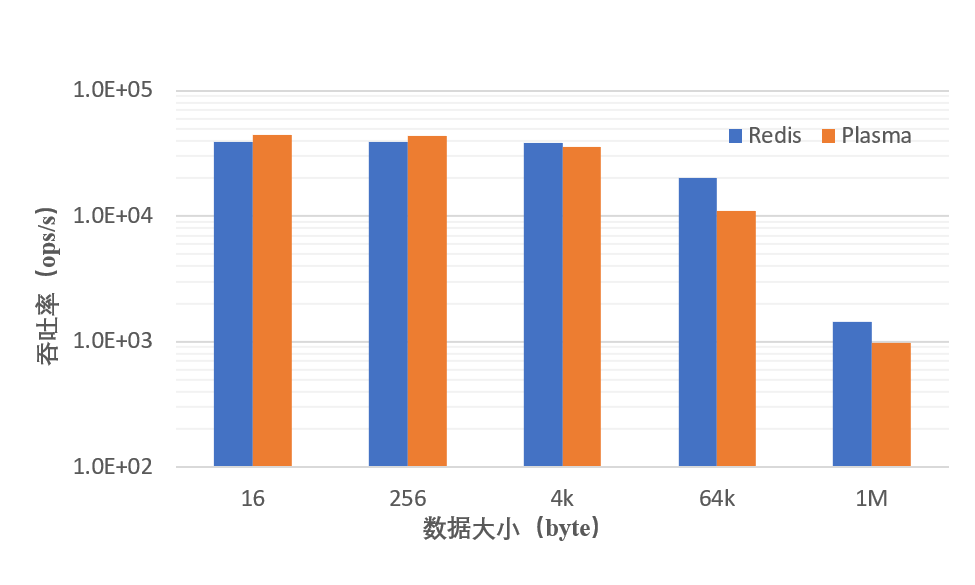
\includegraphics[width=\textwidth]{image/chap02/set.png}
        \caption{Put}
    \end{subfigure}
    \begin{subfigure}{0.49\textwidth}
        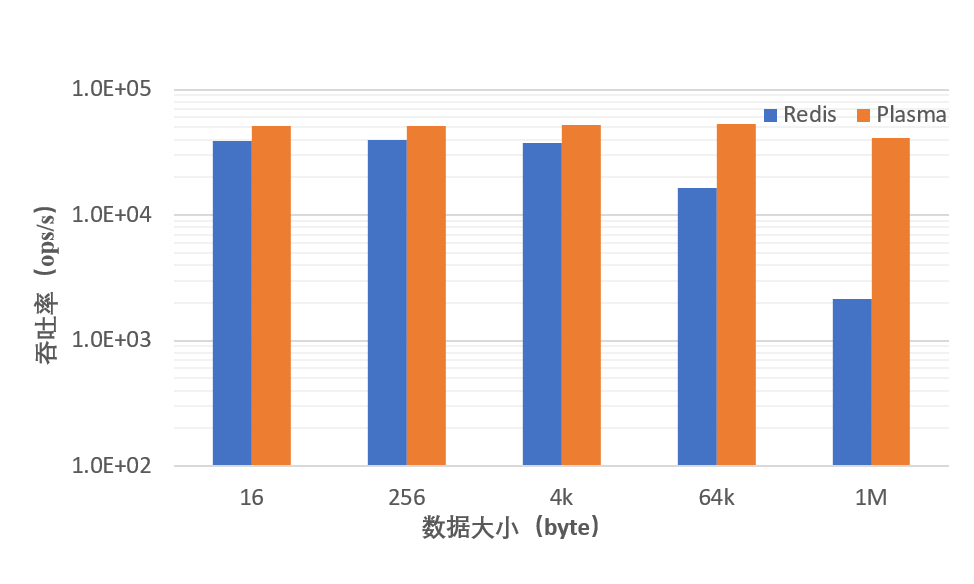
\includegraphics[width=\textwidth]{image/chap02/get.png}
        \caption{Get}
    \end{subfigure}
    \\
    \centering
    \begin{subfigure}{0.49\textwidth}
        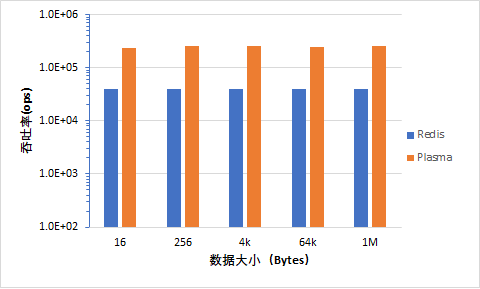
\includegraphics[width=\textwidth]{image/chap02/del.png}
        \caption{Delete}
    \end{subfigure}
    \caption{Redis和Plasma常见操作吞吐对比}
    \label{fig:local_bench}
\end{figure}

如\autoref{fig:local_bench}所示,Plasma单机存储架构的综合性能优于Redis。Plasma和Redis的“put”操作并不相同:对于前者,这一语义实际上是用户通过
调用创建(Create)操作一段分配内存空间,然后将数据对象拷贝到该空间,最终释放(Release)并封存(Seal)对象。可以看到,由于复杂的处理过程,
Plasma在这一操作上有稍高的延迟。由于Plasma通过MMAP机制,在读取操作上支持了零拷贝特性,用户仅需通过IPC接收固定大小的文件描述符,因而在任何数据大小上都具有相似的性能。
相反,Redis使用IPC传输实际数据给用户进程。因此随着数据量增大到1MB,Plasma将对Redis有20倍的性能优势。Plasma和Redis在删除上均拥有常数时间复杂度。

\subsection{数据传输测试}

进一步,我们在两个高性能节点上测试了Plasma和Redis在跨节点数据传输上的吞吐能力。对于Redis,我们在远端节点启动Redis服务器,然后在本地基准测试中重复调用Get操作
进行测试。对于Plasma,在远端节点创建多个数据对象,然后在本地节点调用拉取(Fetch)操作将他们存到本地存储中。

\begin{figure}[h]
    \centering
    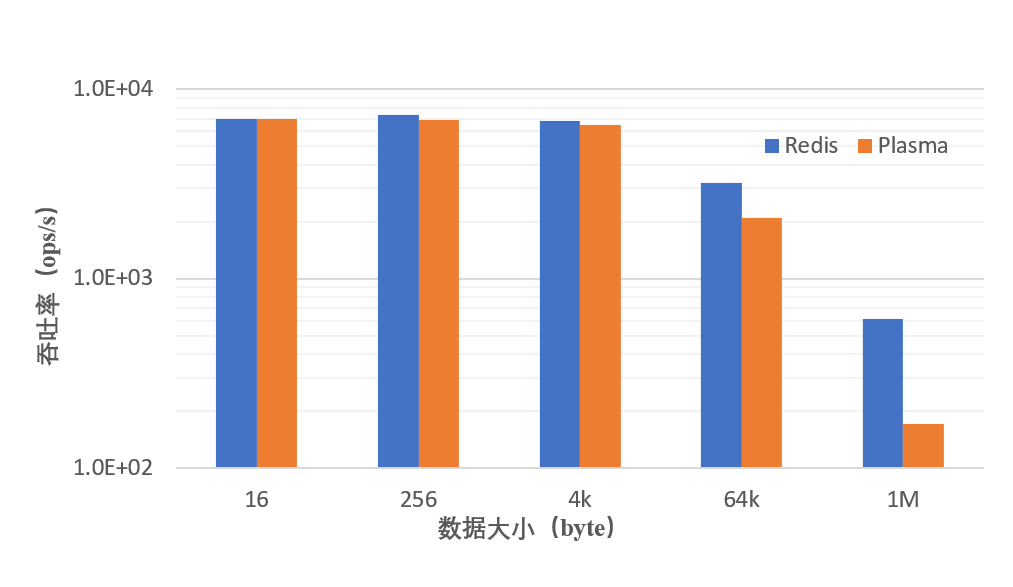
\includegraphics[width=0.7\textwidth]{image/chap02/fetch.png}
    \caption{Redis和Plasma数据传输吞吐对比}
    \label{fig:remote_bench}
\end{figure}

如\autoref{fig:remote_bench}所示,Plasma在远程操作上的吞吐能力显著地劣于Redis,在1MB大小的数据上前者有3.6倍的传输延迟。虽然,两者实际完成的语义很不相同——
Plasma需要先获取对象在集群中的位置,这本身就将访问一次Redis服务器;另外,Plasma发起一次拉取操作包含了一次本地Create操作,这也将产生额外的延迟。而且,
Plasma一次仅以4KB为单位传输数据,也是其在大对象上传输性能明显不如Redis的原因。然而,从我们的实验结果总结来看,不论是Redis还是Plasma都存在明显的性能提升空间:
它们均不能很好地利用超算网络的低延迟和高带宽。特别是支撑分布式计算框架的Plasma,虽然相比Redis等单机数据库实现了分布式,但相当程度地牺牲了较大对象的传输性能,这是原实现没有解决的问题。

因此,这一观察促使我们基于超算网络对Plasma的数据传输机制进行针对性优化。在上述性能测试中,我们已经发现了Plasma在传输大对象时存在非常明显的性能缺陷,因此我们的优化重点应当放在大对象的传输机制上。
不过,小对象的传输对网络延迟敏感,支持RDMA的传输机制也应该能降低其传输延迟。因此,我们希望优化的Plasma实现能够:

\begin{enumerate}
    \item 为较大规模数据的网络传输提供明显更优的传输性能。
    \item 同时,为较小数据的网络传输争取尽可能低的传输延迟。
\end{enumerate}